\chapter{Methodology}
\paragraph{}

This chapter explains how a speech restoration system was built and evaluated using MetricGAN, a leading-edge deep learning model for improving audio quality. Instead of training a model from scratch, this project makes use of a pretrained MetricGAN model integrated into a simple-to-use software tool. This approach makes it possible to restore degraded speech signals without needing extensive computational resources.

The system is a web-based application designed to let users upload audio files that have noise or other distortions, and receive clear, enhanced speech in return. Along with the restored audio, the system also provides audio quality metrics, using the evaluation methods described earlier (such as PESQ, STOI, and SNR).

To help users see the value of modern machine learning, the system compares the quality of the improved audio from the MetricGAN model with the results of a classic Wiener Filter method. This side-by-side comparison gives users a better understanding of how advanced deep learning models perform against traditional approaches for speech restoration.

The frontend of the system, built with the Svelte framework, interacts with a Python-based backend using FastAPI. The backend processes the uploaded audio using the pretrained MetricGAN model from the SpeechBrain library. 

Svelte was chosen for the frontend because it is lightweight and makes building fast, interactive interfaces easy. FastAPI was selected for the backend as it is modern, fast, and works well with Python and machine learning tools. SpeechBrain was used because it provides ready-to-use, high-quality speech enhancement models. This setup makes advanced speech restoration accessible and practical for users, regardless of their technical expertise.

The following sections of this chapter provide more details about how the system is structured, explain the steps involved in processing audio data, describe how the MetricGAN model was integrated, and outline the procedures used to evaluate the system’s performance.

\section{System Overview}

The proposed speech restoration system is designed using a clear client-server structure, making it easy to use and efficient. It consists of two main parts: a user-friendly frontend and a backend processing server. This design enables users to easily access advanced speech enhancement capabilities powered by the MetricGAN model.

\subsection{Frontend (User Interface)}

The frontend is built as a web application using Svelte. It provides a straightforward interface, allowing users to:
\begin{itemize}
    \item Upload speech audio files that are noisy, degraded, or contain missing parts.
    \item View the uploaded audio through clear waveforms and mel-spectrogram visualizations.
    \item Start the audio enhancement process with a simple click.
    \item Listen to or download the restored audio once processed.
\end{itemize}

This design simplifies the user experience, enabling users to test and use advanced audio restoration technologies.


\subsection{Backend (Processing Server)}

The backend server is developed using the Python FastAPI framework. Its responsibilities include:

\begin{itemize}
    \item Receiving audio files from the frontend through HTTP requests.
    \item The server converts the audio to mono and normalizes the amplitude, ensuring consistency for further processing.
    \item Running the pretrained MetricGAN model provided by the SpeechBrain toolkit to enhance the audio.
    \item Waveform and mel spectrogram plots are created using Matplotlib and Librosa to help users visualize the input audio.
    \item Evaluates the audio file quality using the metrics mentioned above (in case the original audio track was uploaded).
    \item Sending the improved audio back and metrics to the frontend.
\end{itemize}


\begin{figure}[htbp]
    \centering
    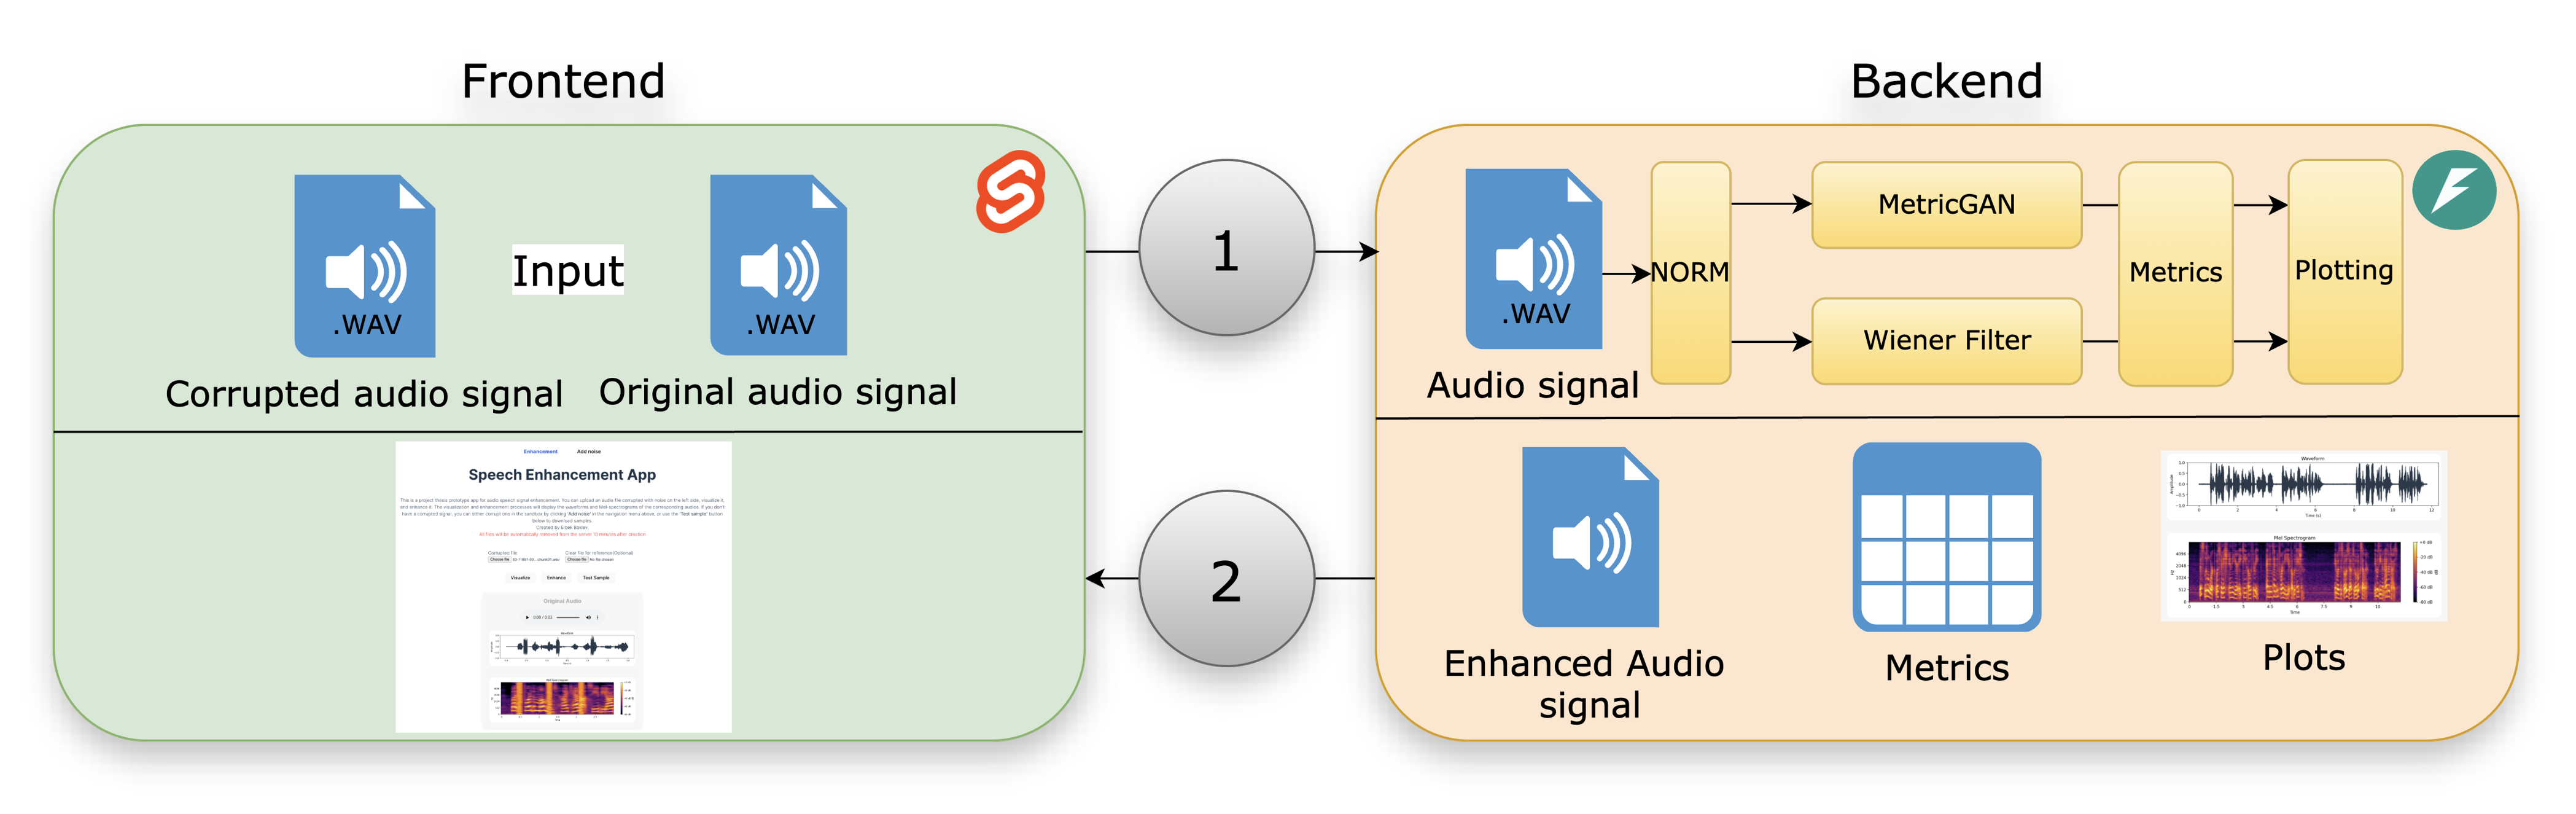
\includegraphics[width=1\linewidth]{figures/sysarch.png}
     \caption{System Architechture}
    \label{fig:figure7}
\end{figure}

Figure \ref{fig:figure7}  illustrates this workflow clearly, showing how the system can be interacted with, and model-based audio restoration is integrated.

\section{MetricGAN Model Details}
 This section summarizes the main architectural components and explains their roles in the speech enhancement process.
 
To better illustrate how MetricGAN works in practice, the core parts of the model’s code are shown in the appendix (see Appendix \ref{appendix:metricgan}) and presented in Figure \ref{fig:figure8}.

\subsection{Generator}
The generator’s job is to take the noisy or degraded audio features and predict what the clean features should look like. In MetricGAN, the generator is a neural network based on bi-directional LSTM layers (see Appendix \ref{appendix:metricgan}, lines 48-54)

\textbf{Input}: The input to the generator is a sequence of features extracted from the noisy audio (typically the magnitude spectrum).

\textbf{Processing:}

\begin{itemize}
    \item The sequence passes through two LSTM layers that capture both past and future context, which is important for modeling speech patterns.
    \item The LSTM output is processed by two fully connected (linear) layers with special initialization (Xavier for weights, zeros for bias).
    \item A custom “learnable sigmoid” activation function helps the network better map its outputs to realistic audio features.
\end{itemize}

\textbf{Output}: The generator predicts a mask or a set of features that can be used to reconstruct the enhanced audio signal.


\subsection{Discriminator}

The discriminator evaluates how close the enhanced output is to the clean reference, but in a way that relates to real perceptual audio quality metrics (see code in Appendix \ref{appendix:metricgan}, lines 77-124).

\textbf{Input}: The discriminator takes both the enhanced (fake) and clean (real) feature representations.

\textbf{Processing:}

\begin{itemize}
    \item The input first goes through batch normalization, followed by four convolutional layers
    \item Four convolutional layers extract spatial patterns from the audio feature maps, with activations and normalization to stabilize training.
    \item The output is averaged over time and frequency to summarize the features.
    \item Three linear layers reduce the dimensionality to a single score, which is used to estimate the perceptual quality (like PESQ).
\end{itemize}

\textbf{Output}: The final output is a single value that approximates the perceptual audio quality metric for the input.


\begin{figure}[htbp]
    \centering
    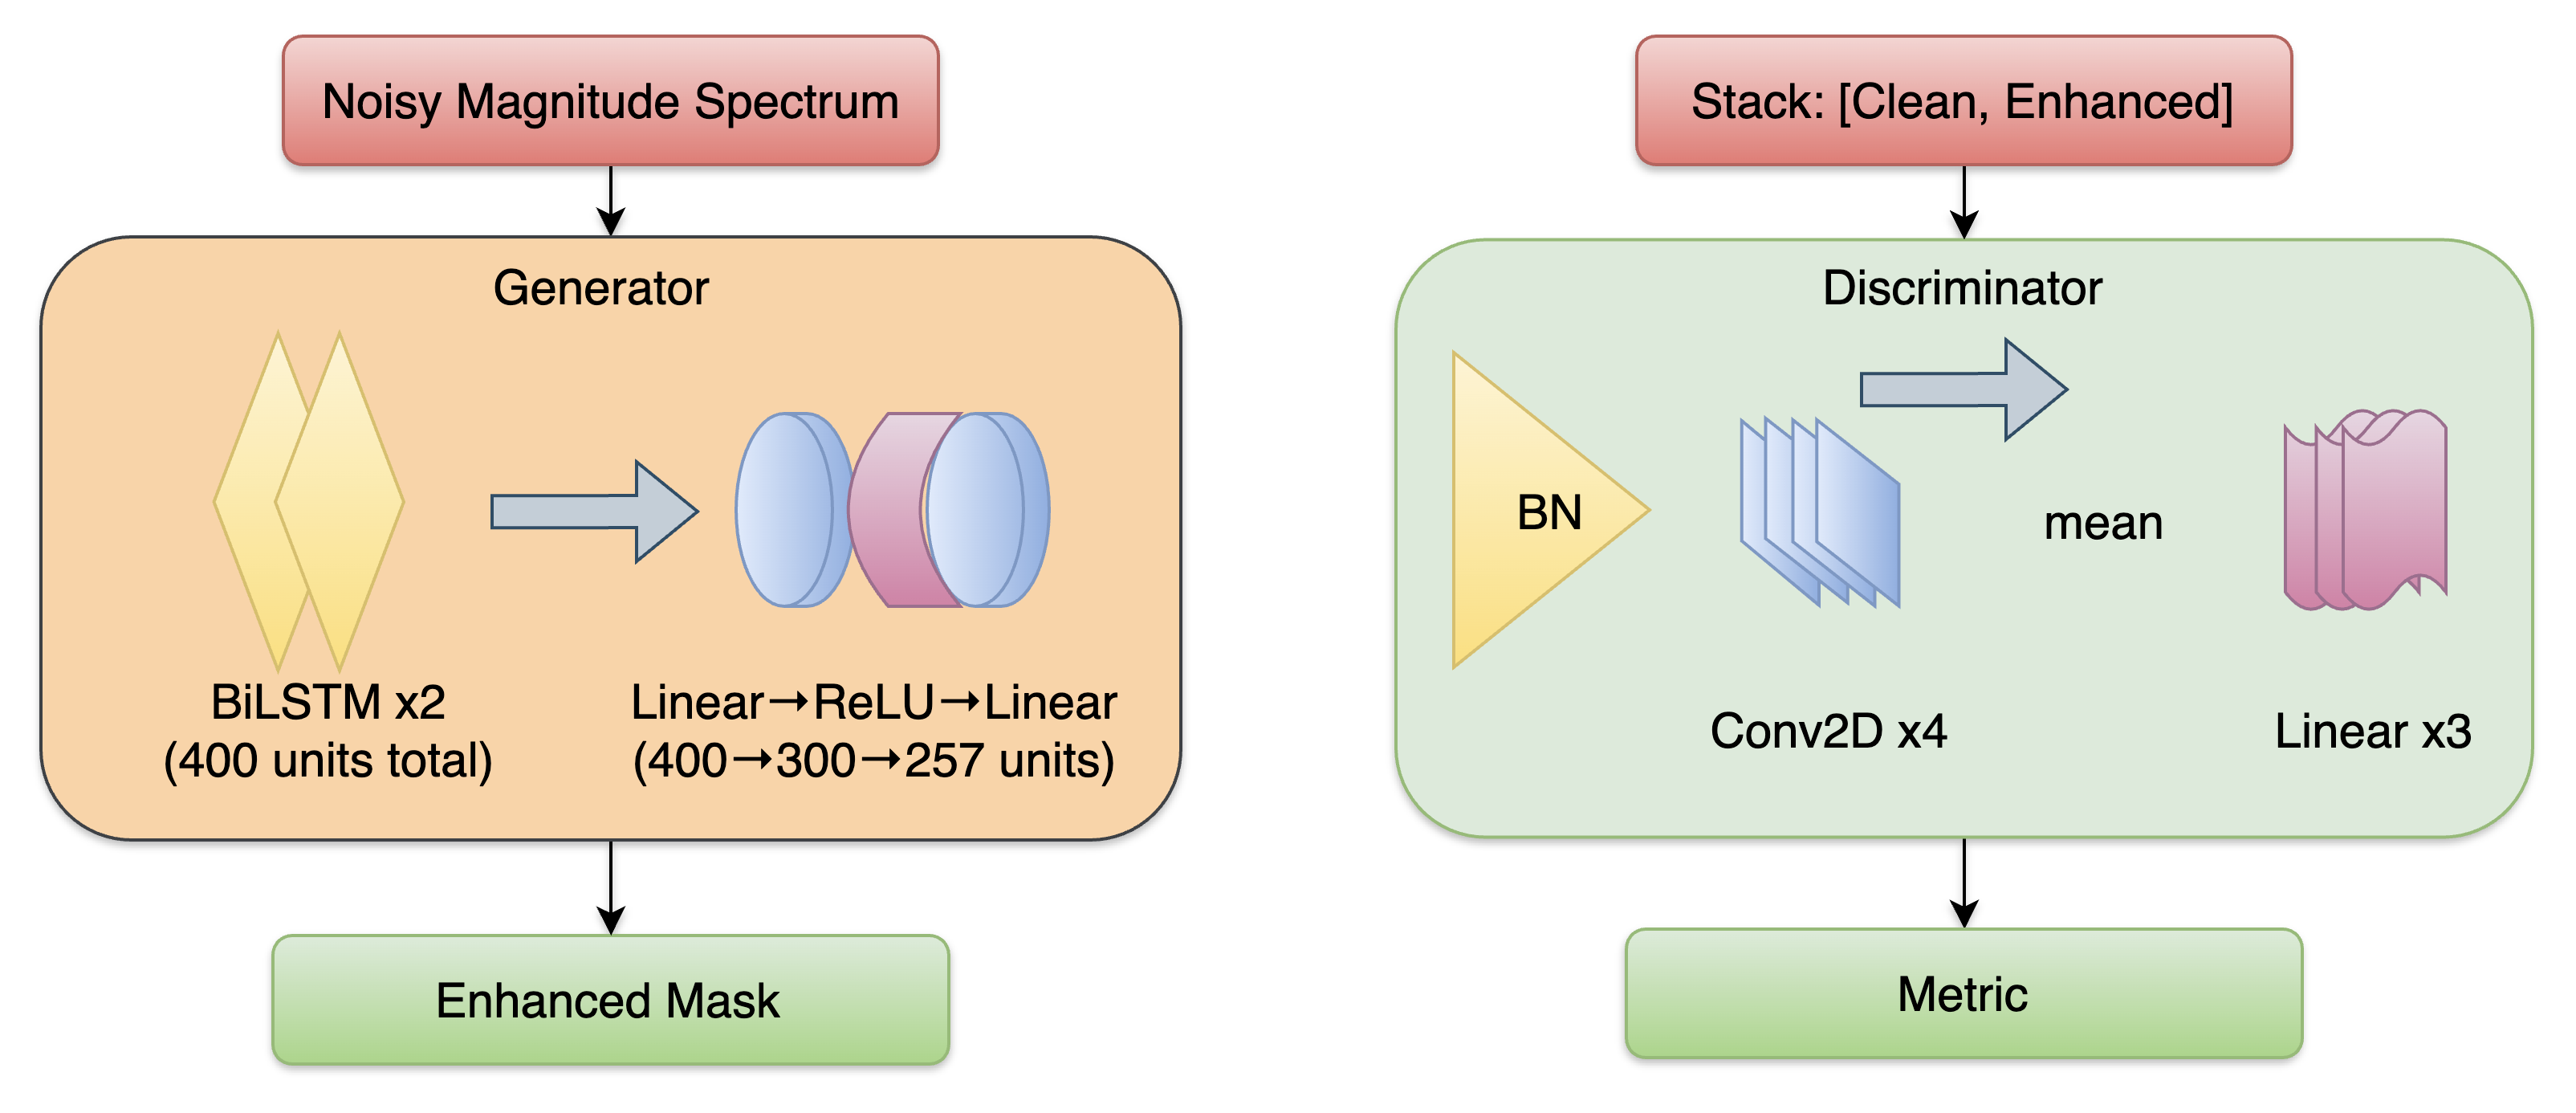
\includegraphics[width=1\linewidth]{figures/MetricGANCodeArch.png}
     \caption{MetricGAN Model Architecture}
    \label{fig:figure8}
\end{figure}


\subsection{Custom Components}

\textbf{Xavier Initialization and Spectral Norm}: The code uses custom helper functions to initialize neural network layers with “Xavier” initialization for weights and zero for biases, and optionally applies spectral normalization (see Appendix \ref{appendix:metricgan}, line 16).

\textbf{Learnable Sigmoid}: This is a special activation function where the “steepness” can be learned by the network, allowing more flexible outputs (see Appendix \ref{appendix:metricgan}, line 26).

\subsection{How the Model is Used in the System}
To use MetricGAN in the application, SpeechBrain’s inference wrapper was used (see Appendix \ref{appendix:metricgan_in_code})

This code loads the pretrained MetricGAN model and its parameters, making it ready for use on any uploaded audio file.

When an audio file is processed, the waveform is passed through the generator to create an enhanced version. During training, the discriminator would provide feedback on the perceptual quality, but for inference (in this project), only the generator is used to clean the audio.



